%  LaTeX support: latex@mdpi.com 
%  For support, please attach all files needed for compiling as well as the log file, and specify your operating system, LaTeX version, and LaTeX editor.

\newcommand{\qsdgst}{General Substrate Theory}
\newcommand{\qsd}{Quantum Substrate Dynamics}
\newcommand{\qsdgsta}{GST}
\newcommand{\qsda}{QSD}

\newcommand{\qsdpapertitle}{Quantum Theory as a Pacing-Limited Regime: Collapse, Coherence, and Causality in General Substrate Theory}
\newcommand{\qsdauthorname}{Michael Bush}
\newcommand{\qsdauthorinitials}{M.B.}
\newcommand{\qsdauthoremail}{mbush@haddentechnologies.com}
\newcommand{\qsdorcid}{0009-0003-9747-9109}
\newcommand{\qsdcorp}{Hadden Technologies Corporation}
\newcommand{\qsdkeywords}{Quantum mechanics, Quantum field theory, Collapse, Causality Interval, Collapse Boundary, Quantum Emission Opportunity, Time symmetry, Entanglement, Quantum Substrate Dynamics}
\newcommand{\qsdmethodstatement}
{This work was developed from first principles, assuming a conserved, Lorentz-invariant coherence substrate. All derivations follow from a single axiom: that physical reality emerges from causal reconfiguration of phase-supported structure. Quantum behavior is modeled as coherence evolution within finite Causality Intervals (CI), ending at Collapse Boundaries (CB), with emission permitted at Quantum Emission Opportunities (QEO). No particles, geometry, or external forces were assumed. The method emphasizes causal closure, time-asymmetric observation, and structural compatibility with known quantum and relativistic limits.}
\newcommand{\qsdabstract}
{Quantum mechanics and quantum field theory (QM/QFT) accurately describe the statistical behavior and field dynamics of microscopic systems, yet remain conceptually incomplete when addressing collapse, measurement, and causality. This work proposes that QM/QFT are valid limiting cases within a broader causal framework---\textit{General
Substrate Theory (GST)}---in which quantum coherence, superposition, and field propagation are constrained by a physically real, Lorentz-compatible substrate.
\\
We introduce the concept of the \textit{coherence tick}, a finite causal interval during which the substrate maintains structured waveforms as real, phase-resolved possibilities. Within this tick, standard QM/QFT formalisms---including unitary evolution, superposition, and entanglement---are fully supported. \textit{This work does not modify quantum equations, but constrains their causal applicability to coherence-supported intervals.} \textit{Collapse is not postulated}, but instead \textit{physically derived as the re-lock event} at the end of the tick: a structural commitment by the substrate that resolves all permissible phase configurations into one irreversible outcome. Measurement is thus reinterpreted not as an observer-triggered event, but as \textit{the first moment post-tick when the committed structure becomes externally accessible}.
\\
This framework preserves all predictive successes of QM/QFT while resolving longstanding interpretive challenges, including the role of the observer, the timing of collapse, and the nature of quantum correlation. The model reinterprets entanglement as \textit{resonant coherence tuning} within a shared substrate mode, constrained by causal propagation (scalar pacing) and phase geometry.
\\
By grounding quantum phenomena in substrate-limited coherence intervals, we unify the statistical reliability of quantum predictions with a deterministic, physically causal substrate mechanism. Collapse and causality are shown to emerge naturally, not through postulates, but through the enforced timing and structural resolution at the core of the substrate itself.}

%%%%%%%%%%%%%%%%%%%%%%%%%%%%%%%%%%%%%%%%%%%%%%%%%%%%%%%%%%%%%%%%%%%%%
\newcommand{\CB}{\mathcal{B}_c}
\newcommand{\CI}{\mathcal{I}_c}
\newcommand{\QEO}{\mathcal{O}_q}
%%%%%%%%%%%%%%%%%%%%%%%%%%%%%%%%%%%%%%%%%%%%%%%%%%%%%%%%%%%%%%%%%%%%%

%=================================================================
\documentclass[preprints,article,submit,pdftex,moreauthors]{Definitions/mdpi} 
%\documentclass[preprints,article,submit,pdftex,moreauthors]{Definitions/mdpi} 
% For posting an early version of this manuscript as a preprint, you may use "preprints" as the journal. Changing "submit" to "accept" before posting will remove line numbers.

% Below journals will use APA reference format:
% admsci, aieduc, behavsci, businesses, econometrics, economies, education, ejihpe, famsci, games, humans, ijcs, ijfs, journalmedia, jrfm, languages, psycholint, publications, tourismhosp, youth

% Below journals will use Chicago reference format:
% arts, genealogy, histories, humanities, jintelligence, laws, literature, religions, risks, socsci

%--------------------
% Class Options:
%--------------------
%----------
% journal
%----------
% Choose between the following MDPI journals:
% accountaudit, acoustics, actuators, addictions, adhesives, admsci, adolescents, aerobiology, aerospace, agriculture, agriengineering, agrochemicals, agronomy, ai, air, algorithms, allergies, alloys, amh, analytica, analytics, anatomia, anesthres, animals, antibiotics, antibodies, antioxidants, applbiosci, appliedchem, appliedmath, appliedphys, applmech, applmicrobiol, applnano, applsci, aquacj, architecture, arm, arthropoda, arts, asc, asi, astronomy, atmosphere, atoms, audiolres, automation, axioms, bacteria, batteries, bdcc, behavsci, beverages, biochem, bioengineering, biologics, biology, biomass, biomechanics, biomed, biomedicines, biomedinformatics, biomimetics, biomolecules, biophysica, biosensors, biosphere, biotech, birds, blockchains, bloods, blsf, brainsci, breath, buildings, businesses, cancers, carbon, cardiogenetics, catalysts, cells, ceramics, challenges, chemengineering, chemistry, chemosensors, chemproc, children, chips, cimb, civileng, cleantechnol, climate, clinbioenerg, clinpract, clockssleep, cmd, cmtr, coasts, coatings, colloids, colorants, commodities, complications, compounds, computation, computers, condensedmatter, conservation, constrmater, cosmetics, covid, crops, cryo, cryptography, crystals, csmf, ctn, curroncol, cyber, dairy, data, ddc, dentistry, dermato, dermatopathology, designs, devices, diabetology, diagnostics, dietetics, digital, disabilities, diseases, diversity, dna, drones, dynamics, earth, ebj, ecm, ecologies, econometrics, economies, education, eesp, ejihpe, electricity, electrochem, electronicmat, electronics, encyclopedia, endocrines, energies, eng, engproc, ent, entomology, entropy, environments, epidemiologia, epigenomes, esa, est, famsci, fermentation, fibers, fintech, fire, fishes, fluids, foods, forecasting, forensicsci, forests, fossstud, foundations, fractalfract, fuels, future, futureinternet, futureparasites, futurepharmacol, futurephys, futuretransp, galaxies, games, gases, gastroent, gastrointestdisord, gastronomy, gels, genealogy, genes, geographies, geohazards, geomatics, geometry, geosciences, geotechnics, geriatrics, glacies, grasses, greenhealth, gucdd, hardware, hazardousmatters, healthcare, hearts, hemato, hematolrep, heritage, higheredu, highthroughput, histories, horticulturae, hospitals, humanities, humans, hydrobiology, hydrogen, hydrology, hygiene, idr, iic, ijerph, ijfs, ijgi, ijmd, ijms, ijns, ijpb, ijt, ijtm, ijtpp, ime, immuno, informatics, information, infrastructures, inorganics, insects, instruments, inventions, iot, j, jal, jcdd, jcm, jcp, jcs, jcto, jdad, jdb, jeta, jfb, jfmk, jimaging, jintelligence, jlpea, jmahp, jmmp, jmms, jmp, jmse, jne, jnt, jof, joitmc, joma, jop, jor, journalmedia, jox, jpbi, jpm, jrfm, jsan, jtaer, jvd, jzbg, kidney, kidneydial, kinasesphosphatases, knowledge, labmed, laboratories, land, languages, laws, life, lights, limnolrev, lipidology, liquids, literature, livers, logics, logistics, lubricants, lymphatics, machines, macromol, magnetism, magnetochemistry, make, marinedrugs, materials, materproc, mathematics, mca, measurements, medicina, medicines, medsci, membranes, merits, metabolites, metals, meteorology, methane, metrics, metrology, micro, microarrays, microbiolres, microelectronics, micromachines, microorganisms, microplastics, microwave, minerals, mining, mmphys, modelling, molbank, molecules, mps, msf, mti, multimedia, muscles, nanoenergyadv, nanomanufacturing, nanomaterials, ncrna, ndt, network, neuroglia, neurolint, neurosci, nitrogen, notspecified, nursrep, nutraceuticals, nutrients, obesities, oceans, ohbm, onco, oncopathology, optics, oral, organics, organoids, osteology, oxygen, parasites, parasitologia, particles, pathogens, pathophysiology, pediatrrep, pets, pharmaceuticals, pharmaceutics, pharmacoepidemiology, pharmacy, philosophies, photochem, photonics, phycology, physchem, physics, physiologia, plants, plasma, platforms, pollutants, polymers, polysaccharides, populations, poultry, powders, preprints, proceedings, processes, prosthesis, proteomes, psf, psych, psychiatryint, psychoactives, psycholint, publications, purification, quantumrep, quaternary, qubs, radiation, reactions, realestate, receptors, recycling, regeneration, religions, remotesensing, reports, reprodmed, resources, rheumato, risks, robotics, rsee, ruminants, safety, sci, scipharm, sclerosis, seeds, sensors, separations, sexes, signals, sinusitis, siuj, skins, smartcities, sna, societies, socsci, software, soilsystems, solar, solids, spectroscj, sports, standards, stats, std, stresses, surfaces, surgeries, suschem, sustainability, symmetry, synbio, systems, tae, targets, taxonomy, technologies, telecom, test, textiles, thalassrep, therapeutics, thermo, timespace, tomography, tourismhosp, toxics, toxins, transplantology, transportation, traumacare, traumas, tropicalmed, universe, urbansci, uro, vaccines, vehicles, venereology, vetsci, vibration, virtualworlds, viruses, vision, waste, water, wem, wevj, wild, wind, women, world, youth, zoonoticdis

%---------
% article
%---------
% The default type of manuscript is "article", but can be replaced by: 
% abstract, addendum, article, benchmark, book, bookreview, briefcommunication, briefreport, casereport, changes, clinicopathologicalchallenge, comment, commentary, communication, conceptpaper, conferenceproceedings, correction, conferencereport, creative, datadescriptor, discussion, entry, expressionofconcern, extendedabstract, editorial, essay, erratum, fieldguide, hypothesis, interestingimages, letter, meetingreport, monograph, newbookreceived, obituary, opinion, proceedingpaper, projectreport, reply, retraction, review, perspective, protocol, shortnote, studyprotocol, supfile, systematicreview, technicalnote, viewpoint, guidelines, registeredreport, tutorial,  giantsinurology, urologyaroundtheworld
% supfile = supplementary materials

%----------
% submit
%----------
% The class option "submit" will be changed to "accept" by the Editorial Office when the paper is accepted. This will only make changes to the frontpage (e.g., the logo of the journal will get visible), the headings, and the copyright information. Also, line numbering will be removed. Journal info and pagination for accepted papers will also be assigned by the Editorial Office.

%------------------
% moreauthors
%------------------
% If there is only one author the class option oneauthor should be used. Otherwise use the class option moreauthors.

%---------
% pdftex
%---------
% The option pdftex is for use with pdfLaTeX. Remove "pdftex" for (1) compiling with LaTeX & dvi2pdf (if eps figures are used) or for (2) compiling with XeLaTeX.

%=================================================================
% MDPI internal commands - do not modify
\firstpage{1} 
\makeatletter 
\setcounter{page}{\@firstpage} 
\makeatother
\pubvolume{1}
\issuenum{1}
\articlenumber{0}
\pubyear{2025}
\copyrightyear{2025}
%\externaleditor{Firstname Lastname} % More than 1 editor, please add `` and '' before the last editor name
\datereceived{ } 
\daterevised{ } % Comment out if no revised date
\dateaccepted{ } 
\datepublished{ } 
%\datecorrected{} % For corrected papers: "Corrected: XXX" date in the original paper.
%\dateretracted{} % For retracted papers: "Retracted: XXX" date in the original paper.
\hreflink{https://doi.org/} % If needed use \linebreak
%\doinum{}
%\pdfoutput=1 % Uncommented for upload to arXiv.org
%\CorrStatement{yes}  % For updates
%\longauthorlist{yes} % For many authors that exceed the left citation part

%=================================================================
% Add packages and commands here. The following packages are loaded in our class file: fontenc, inputenc, calc, indentfirst, fancyhdr, graphicx, epstopdf, lastpage, ifthen, float, amsmath, amssymb, lineno, setspace, enumitem, mathpazo, booktabs, titlesec, etoolbox, tabto, xcolor, colortbl, soul, multirow, microtype, tikz, totcount, changepage, attrib, upgreek, array, tabularx, pbox, ragged2e, tocloft, marginnote, marginfix, enotez, amsthm, natbib, hyperref, cleveref, scrextend, url, geometry, newfloat, caption, draftwatermark, seqsplit
% cleveref: load \crefname definitions after \begin{document}

\usepackage{tikz}
\usetikzlibrary{angles, quotes}
\usepackage{pgfplots}
\pgfplotsset{compat=1.17}
 \usetikzlibrary{calc}
%=================================================================
% Please use the following mathematics environments: Theorem, Lemma, Corollary, Proposition, Characterization, Property, Problem, Example, ExamplesandDefinitions, Hypothesis, Remark, Definition, Notation, Assumption
%% For proofs, please use the proof environment (the amsthm package is loaded by the MDPI class).

%=================================================================
% Full title of the paper (Capitalized)
\Title{\qsdpapertitle}


% MDPI internal command: Title for citation in the left column
\TitleCitation{Title}

% Author Orchid ID: enter ID or remove command
\newcommand{\orcidauthorA}{\qsdorcid} % Add \orcidA{} behind the author's name
%\newcommand{\orcidauthorB}{0000-0000-0000-000X} % Add \orcidB{} behind the author's name

% Authors, for the paper (add full first names)
\Author{\qsdauthorname $^{1}$\orcidA{}}

%\longauthorlist{yes}

% MDPI internal command: Authors, for metadata in PDF
\AuthorNames{\qsdauthorname}

% MDPI internal command: Authors, for citation in the left column, only choose below one of them according to the journal style
% If this is a Chicago style journal 
% (arts, genealogy, histories, humanities, jintelligence, laws, literature, religions, risks, socsci): 
% Lastname, Firstname, Firstname Lastname, and Firstname Lastname.

% If this is a APA style journal 
% (admsci, behavsci, businesses, econometrics, economies, education, ejihpe, games, humans, ijfs, journalmedia, jrfm, languages, psycholint, publications, tourismhosp, youth): 
% Lastname, F., Lastname, F., \& Lastname, F.

% If this is a ACS style journal (Except for the above Chicago and APA journals, all others are in the ACS format): 
% Lastname, F.; Lastname, F.; Lastname, F.
\isAPAStyle{%
       \AuthorCitation{Lastname, F., Lastname, F., \& Lastname, F.}
         }{%
        \isChicagoStyle{%
        \AuthorCitation{Lastname, Firstname, Firstname Lastname, and Firstname Lastname.}
        }{
        \AuthorCitation{Lastname, F.; Lastname, F.; Lastname, F.}
        }
}

% Affiliations / Addresses (Add [1] after \address if there is only one affiliation.)
\address{%
$^{1}$ \quad \qsdcorp; \qsdauthoremail\\
%$^{2}$ \quad Affiliation 2; e-mail@e-mail.com
}

% Contact information of the corresponding author
\corres{Correspondence: \qsdauthoremail (\qsdauthorinitials)}

% Current address and/or shared authorship
%\firstnote{Shiloh, IL: Independent Researcher.}  % Current address should not be the same as any items in the Affiliation section.
%\secondnote{These authors contributed equally to this work.}
% The commands \thirdnote{} till \eighthnote{} are available for further notes

%\simplesumm{} % Simple summary

%\conference{} % An extended version of a conference paper


% Abstract (Do not insert blank lines, i.e. \\) 
\abstract{\qsdabstract}

% Keywords
\keyword{\qsdkeywords} 

% The fields PACS, MSC, and JEL may be left empty or commented out if not applicable
%\PACS{J0101}
%\MSC{}
%\JEL{}

%%%%%%%%%%%%%%%%%%%%%%%%%%%%%%%%%%%%%%%%%%
% Only for the journal Diversity
%\LSID{\url{http://}}

%%%%%%%%%%%%%%%%%%%%%%%%%%%%%%%%%%%%%%%%%%
% Only for the journal Applied Sciences
%\featuredapplication{Authors are encouraged to provide a concise description of the specific application or a potential application of the work. This section is not mandatory.}
%%%%%%%%%%%%%%%%%%%%%%%%%%%%%%%%%%%%%%%%%%

%%%%%%%%%%%%%%%%%%%%%%%%%%%%%%%%%%%%%%%%%%
% Only for the journal Data
%\dataset{DOI number or link to the deposited data set if the data set is published separately. If the data set shall be published as a supplement to this paper, this field will be filled by the journal editors. In this case, please submit the data set as a supplement.}
%\datasetlicense{License under which the data set is made available (CC0, CC-BY, CC-BY-SA, CC-BY-NC, etc.)}

%%%%%%%%%%%%%%%%%%%%%%%%%%%%%%%%%%%%%%%%%%
% Only for the journal BioTech, Fishes, Neuroimaging and Toxins
%\keycontribution{The breakthroughs or highlights of the manuscript. Authors can write one or two sentences to describe the most important part of the paper.}

%%%%%%%%%%%%%%%%%%%%%%%%%%%%%%%%%%%%%%%%%%
% Only for the journal Encyclopedia
%\encyclopediadef{For entry manuscripts only: please provide a brief overview of the entry title instead of an abstract.}

%%%%%%%%%%%%%%%%%%%%%%%%%%%%%%%%%%%%%%%%%%
% Only for the journal Advances in Respiratory Medicine, Future, Sensors and Smart Cities
%\addhighlights{yes}
%\renewcommand{\addhighlights}{%
%
%\noindent This is an obligatory section in ``Advances in Respiratory Medicine'', ``Future'', ``Sensors'' and ``Smart Cities”, whose goal is to increase the discoverability and readability of the article via search engines and other scholars. Highlights should not be a copy of the abstract, but a simple text allowing the reader to quickly and simplified find out what the article is about and what can be cited from it. Each of these parts should be devoted up to 2~bullet points.\vspace{3pt}\\
%\textbf{What are the main findings?}
% \begin{itemize}[labelsep=2.5mm,topsep=-3pt]
% \item First bullet.
% \item Second bullet.
% \end{itemize}\vspace{3pt}
%\textbf{What is the implication of the main finding?}
% \begin{itemize}[labelsep=2.5mm,topsep=-3pt]
% \item First bullet.
% \item Second bullet.
% \end{itemize}
%}

%%%%%%%%%%%%%%%%%%%%%%%%%%%%%%%%%%%%%%%%%%
\begin{document}
%%%%%%%%%%%%%%%%%%%%%%%%%%%%%%%%%%%%%%%%%%
% The order of the section titles is different for some journals. Please refer to the "Instructions for Authors” on the journal homepage.

%%%%%%%%%%%%%%%%%%%%%%%%%%%%%%%%%%%%%%%%%%
\section{Introduction}
%%%%%%%%%%%%%%%%%%%%%%%%%%%%%%%%%%%%%%%%%%

Quantum mechanics (QM) and quantum field theory (QFT) offer powerful and precise frameworks for describing the statistical structure of microscopic systems. Their formalism has produced predictions of extraordinary accuracy and technologies of increasing sophistication. Yet persistent conceptual questions remain unresolved: What is the physical status of the wavefunction? What causes collapse, and when does it occur? Why does measurement produce irreversible outcomes if the underlying equations are time-symmetric?

These questions arise not from flaws in the mathematical formalism, but from the absence of a clearly defined causal structure. Quantum systems evolve unitarily under the Schrödinger equation, but this evolution terminates abruptly when a measurement is made. The standard theory provides no internal mechanism for this transition. In QFT, the issue is displaced into operator algebra and vacuum excitation, but the core ambiguity remains: what physically distinguishes the domain of reversible wavefunction evolution from the moment of irreversible outcome?

This work proposes that QM and QFT are not incorrect, but physically incomplete. We introduce a physically grounded coherence framework—\textit{\qsdgst (\qsdgsta)}~\cite{bush-gst}—in which quantum behavior arises as a limiting case within discrete, causally permitted coherence intervals. These spans, called \textit{Causality Intervals (CI)}, define the maximum duration over which a wavefunction or field excitation may evolve coherently before requiring structural resolution. At the end of each CI lies a \textit{Collapse Boundary (CB)}, where the substrate irreversibly re-locks the system's configuration. If this resolution entails energy, tension, or waveform offload, it produces a \textit{Quantum Emission Opportunity (QEO)}—a physically grounded alternative to axiomatic measurement.

This framework preserves all predictions of QM and QFT while providing a physical mechanism for collapse, emission, and entanglement. Wavefunctions, superpositions, and fields are real—but only within the CI, where coherence is supported. Collapse is not triggered by observation, but by causal exhaustion of the interval. Entanglement is not instantaneous linkage, but resonance tuning: structures formed within the same coherence envelope remain phase-compatible and may respond to serialized emissions if their tick pacing remains aligned. These emissions do not enforce collapse in the partner structure, but may stimulate a re-lock if coherence conditions permit.

A key outcome of this framing is a resolution to the quantum time symmetry paradox. Within the CI, time evolution is forward and fully reversible: the system experiences \( +t \) as internal phase structure unfolds. But collapse marks the end of that frame. From the observer’s point of view, measurement accesses only the committed result—forcing any reconstruction of internal evolution to occur retrospectively in \( -t \). Time symmetry is preserved in the system, but broken at the level of observation. This distinction resolves the apparent contradiction between reversible quantum dynamics and irreversible measurement.

In what follows, we define this framework and show that it not only preserves the core mathematics of quantum theory, but also anchors it in a causal structure that explains why collapse, measurement, and correlation occur as they do—without mystery, paradox, or metaphysical ambiguity. \qsd (\qsda)~\cite{bush2025}, is the dynamic expression of \qsdgsta, reframes the quantum formalism not as a complete description of reality, but as the domain-specific language of coherence playing out within a deeper causal substrate.

%%%%%%%%%%%%%%%%%%%%%%%%%%%%%%%%%%%%%%%%%%
\section{Materials and Methods}
%%%%%%%%%%%%%%%%%%%%%%%%%%%%%%%%%%%%%%%%%%
\qsdmethodstatement
\\
\\
The use of AI is disclosed in alignment with journal policy for transparency in the writing process as presented below:\\
\begin{itemize}
    \item All core theoretical work was developed independently from first principles. AI systems (ChatGPT, Grok and ScholarGPT) were used solely to identify points of ambiguity, implicit assumptions, or language that could lead to misunderstanding. These systems were treated as simulated reviewers, offering adversarial or skeptical feedback. Clarifications and refinements were incorporated where needed to ensure clarity, coherence, and interpretive precision. No AI-generated content contributed to the construction of the theoretical model itself. OpenAI’s ChatGPT (version GPT-4o, 2025)  was used for editorial and formatting processes.
\end{itemize}



%%%%%%%%%%%%%%%%%%%%%%%%%%%%%%%%%%%%%%%%%%
%\section{Results}

%%%%%%%%%%%%%%%%%%%%%%%%%%%%%%%%%%%%%%%%%%
\section{Discussion}
%%%%%%%%%%%%%%%%%%%%%%%%%%%%%%%%%%%%%%%%%%
\subsection{Substrate Causality and Coherence Foundations}
\label{sec:substratefoundation}

The causal structure proposed in this work is grounded in the concept of a conserved, phase-supporting substrate that governs when and how quantum behavior is physically permitted. Rather than postulating an abstract Hilbert space in which states evolve indefinitely, we define a coherence-capable substrate that imposes strict temporal and geometric constraints on superposition, entanglement, and collapse. These constraints take the form of discrete causal windows—finite intervals during which coherent evolution is supported—followed by irreversible re-locking events that commit phase structure into a measurable outcome.

This section introduces the three core causal components of the framework: the \textit{Causality Interval} (CI), the \textit{Collapse Boundary} (CB), and the \textit{Quantum Emission Opportunity} (QEO). Together, they form the minimal substrate cycle over which quantum structure can evolve, resolve, and (when permitted) emit. These components replace observer-centric and axiomatically postulated collapse mechanisms with internal causal processes that respect both quantum mathematics and relativistic timing.

\subsubsection{The General Substrate Framework}

We begin by positing the existence of a globally conserved coherence field—the substrate—that supports all physical structure through localized phase configuration. This substrate is not an empty vacuum, nor a background spacetime, but a Lorentz-compatible medium that defines when and where physical structure may form and persist. Evolution within this substrate does not imply motion in space, but reconfiguration of phase under local causal constraints. Coherence is not free—it must be supported.

The coherence capacity of the substrate is finite. It supports coherent structures over a limited spatial extent \( L_{\text{coh}} \) and for a finite duration determined by the scalar pacing velocity \( c_s \). This gives rise to a causally defined interval during which structure may evolve reversibly before collapse becomes compulsory. The substrate’s coherence limits are not imposed from outside but arise from its own phase load and propagation characteristics.

\subsubsection{The Causality Interval (CI)}

A \textit{Causality Interval} (CI), denoted \( \mathcal{I}_c \), is the maximal duration over which a coherent phase structure may evolve under unitary conditions without being forced to commit to a definite outcome. This interval defines the domain of validity for quantum mechanics and field theory: within it, wavefunctions are physically real, interference is supported, and entanglement correlations may persist. The coherence interval is bounded by:

\[
t_{\text{CI}} = \frac{L_{\text{coh}}}{c_s}
\]

where \( L_{\text{coh}} \) is the spatial coherence envelope of the structure, and \( c_s \) is the scalar recovery velocity of the substrate. Notably, \( L_{\text{coh}} \) is not a universal constant. It varies with local substrate tension, geometry, and phase stress. As such, coherence intervals are dynamic, and \( L_{\text{coh}} \neq L_{\text{coh}} \) across different systems or even across time for the same system.

During the CI, internal evolution is forward in time (\( +t \)) from the perspective of the structure. The wavefunction develops its internal geometry under full superposition. However, from the external perspective of an observer, that evolution is inaccessible until collapse occurs. After collapse, any reconstruction of internal structure must be performed retrospectively using \( -t \). This dual perspective resolves the time symmetry paradox: both time directions are valid, but causally constrained to their respective frames.

\subsubsection{The Collapse Boundary (CB)}

The \textit{Collapse Boundary}, denoted \( \mathcal{B}_c \), is the terminal point of a coherence interval. At this boundary, the substrate must resolve the coherent structure it has supported and re-lock it into a committed, irreversible configuration. Collapse is not externally triggered by measurement—it is the result of coherence expiration. At the CB, the substrate selects a single structurally permissible phase configuration and commits to it.

Importantly, this collapse is not the annihilation of structure. It is the conclusion of a specific configuration. If the coherence geometry permits, the structure may persist into a future interval under new conditions. Collapse is thus not destruction—it is a causal gate. Measurement becomes possible only after this gate is crossed, when the structure has become stable and externally accessible.

\subsubsection{The Quantum Emission Opportunity (QEO)}

When collapse involves the release of energy, mass, or phase tension, the substrate triggers a \textit{Quantum Emission Opportunity} (QEO), denoted \( \mathcal{E}_q \). The QEO is a subset of collapse events in which the internal phase geometry is serialized—projected into the substrate as a wave or field structure. This serialized emission is the causal mechanism behind photons, radiation, and spectral quantization. It replaces the need for probabilistic emission or quantum jumps.

Only complete, phase-consistent geometries may serialize. Partial or out-of-phase configurations cannot emit. The resulting spectral lines or emission features reflect the internal geometry of the structure—not as statistical probabilities, but as structured collapses constrained by coherence boundaries. The QEO is not a requirement—it is a permission. Many collapses produce no emission, while some may stimulate tuned partners to re-lock in correlated responses.

\smallskip

In total, the CI–CB–QEO cycle defines the minimal causal unit of quantum evolution. The wavefunction exists within the CI, is resolved at the CB, and may emit at the QEO. Collapse does not destroy structure—it localizes and re-locks it. Time symmetry exists within the CI; irreversibility begins at the CB. Observation is not a trigger, but a consequence of causal finality.

\begin{figure}[h!]
\centering
\begin{tikzpicture}[>=stealth, node distance=4.7cm, every node/.style={font=\small}, align=center]

% Nodes
\node (ci) [draw, rounded corners, minimum width=3.8cm, minimum height=1.2cm, fill=blue!10] {\textbf{Causality Interval} \\ \( \mathcal{I}_c \)};
\node (cb) [right of=ci, draw, rounded corners, minimum width=4.1cm, minimum height=1.2cm, fill=orange!15] {\textbf{Collapse Boundary} \\ \( \mathcal{B}_c \)};
\node (qeo) [right of=cb, draw, rounded corners, minimum width=4.3cm, minimum height=1.2cm, fill=red!10] {\textbf{Quantum Emission Opportunity} \\ \( \mathcal{E}_q \)};

% Arrows
\draw[->, thick] (ci) -- (cb) node[midway, above, yshift=2.0em] {\footnotesize evolution ends};
\draw[->, thick] (cb) -- (qeo) node[midway, above, yshift=2.0em] {\footnotesize if offload required};

% Labels under nodes
\node at ($(ci.south) + (0,-0.3)$) {\footnotesize quantum evolution (unitary)};
\node at ($(cb.south) + (0,-0.3)$) {\footnotesize structure re-locks};
\node at ($(qeo.south) + (0,-0.3)$) {\footnotesize serialized emission};

\end{tikzpicture}
\caption{CI–CB–QEO sequence within a coherence frame. Quantum behavior occurs within the Causality Interval \( \mathcal{I}_c \), terminates at the Collapse Boundary \( \mathcal{B}_c \), and may emit a signal at the Quantum Emission Opportunity \( \mathcal{E}_q \).}
\label{fig:cicbqeo}
\end{figure}


%@%%%%%%%%%%%%%%%%%%%%%%%%%%%%%%%%%%%%%%%%
\subsection{Quantum Mechanics Within the CI}
\label{subsec:qminci}

Within each Causality Interval \( \mathcal{I}_c \), quantum mechanical and quantum field-theoretic behavior unfold as valid, physically permitted structures supported by the coherence properties of the substrate. During this interval, the substrate maintains a stable internal phase geometry, allowing for the full expression of superposition, interference, entanglement, and field excitation as real and reversible dynamics. The standard quantum formalism applies exactly—but only within the temporal and structural bounds defined by \( \mathcal{I}_c \).

\subsubsection{Validity of QM and QFT Formulations}

Standard quantum mechanics assumes continuous unitary evolution until interrupted by measurement. In the QSD framework, this unitary behavior is correct—but is only physically permitted within the span of a coherence interval. The substrate supports coherent phase evolution for a finite duration, constrained by the local coherence envelope \( L_{\text{coh}} \) and scalar pacing velocity \( c_s \). No external observer, detector, or environmental decoherence is required to end this evolution; it concludes naturally as the substrate reaches its causal limit.

All core features of QM and QFT—Schrödinger evolution, Hilbert superposition, Fock space excitations—are structurally valid while the substrate remains coherent. The mathematics remains unchanged; only the causal domain in which that mathematics applies is newly defined.

This framework does not modify quantum mechanics, but situates its validity within a structurally defined domain. The substrate defines when coherence evolution is supported — not whether the quantum equations are correct.
%%%%%%%%%%%%%

\subsubsection{Collapse Without Axioms}

In the standard formalism, collapse is postulated to occur upon observation, often with no identified physical mechanism. In QSD, collapse arises inevitably and causally at the end of each \( \mathcal{I}_c \), as the substrate reaches its structural boundary. This moment, marked by the Collapse Boundary \( \mathcal{B}_c \), is not an external intervention—it is a re-locking event internal to the substrate, in which a single coherent configuration is selected from the available phase structure.

Importantly, collapse in this framework is not destructive. It terminates the current coherence window but does not annihilate the structure. If the underlying waveform remains coherent and structurally supported, it may re-emerge in a new \( \mathcal{I}_c \) under different causal constraints. Collapse thus marks the resolution of a frame, not the end of the object.

\subsubsection{Why the Math Remains Valid}

QSD does not modify or challenge the mathematical structure of quantum theory. Instead, it situates that structure within a physically grounded causal boundary. The wavefunction is reinterpreted as a phase-resolved coherence geometry valid only within \( \mathcal{I}_c \). Probabilities arise not from ontological indeterminacy, but from structural projection: when collapse occurs at \( \mathcal{B}_c \), only certain configurations are compatible with the substrate's causal geometry, and these are selected through resonance and symmetry filtering.

The Born rule, interference, entanglement correlations, and operator formalism remain mathematically intact. What QSD adds is a causal interpretation: quantum statistics are not abstract—they are the measurable outcomes of structured phase evolution subject to finite causal permission.

\smallskip

In summary, quantum mechanics and field theory are recovered in full as the effective description of structures evolving within a coherence-bound domain. Collapse is not a paradox—it is a structural necessity. Measurement is not a trigger—it is a consequence. The wavefunction is not a mystical possibility cloud—it is a temporally gated, phase-resolved coherence geometry whose evolution is real, but causally finite.


%%%%%%%%%%%%%%%%%%%%%%%%%%%%%%%%%%%%%%%%%%
\subsection{Entanglement as Resonant Correlation}
\label{subsec:entanglement}

Quantum entanglement has long been regarded as one of the most paradoxical phenomena in physics—giving rise to nonlocal correlations that appear to defy causal structure, signal locality, or any classical notion of independence. In the standard quantum formalism, entangled systems are described by composite wavefunctions that evolve jointly until collapse occurs, at which point the state of one subsystem appears to instantaneously determine the state of its partner, regardless of spatial separation.

In the QSD framework, entanglement is reinterpreted not as linkage, but as a consequence of \textit{resonant coherence tuning}. Structures that emerge within the same coherence envelope \( L_{\text{coh}} \) during a shared Causality Interval \( \mathcal{I}_c \) inherit a common phase geometry and scalar pacing. Their ability to respond to one another’s collapse events arises not from superluminal connection, but from physical compatibility and synchronized causal access within a coherence-bound domain.

\subsubsection{Shared Tuning, Not Linkage}

Entangled systems in QSD are phase-compatible structures that share a common substrate tuning—established during their formation within the same \( L_{\text{coh}} \) region. Their internal waveforms are coherent in both geometry and tick pacing, which allows them to respond to one another’s collapse emissions if both remain within the same coherence framework.

This coherence-based tuning replaces the need for metaphysical collapse or instantaneous state determination. The apparent correlation between measurement outcomes arises because both systems are still resonant with the same internal structure—until one or both lose alignment due to phase drift or causal exit.

\subsubsection{Collapse Serialization and Resonant Response}

When one structure reaches the Collapse Boundary \( \mathcal{B}_c \) and triggers a Quantum Emission Opportunity \( \mathcal{E}_q \), its internal coherence geometry is serialized into a scalar waveform. This serialized projection propagates causally through the substrate and reflects the structure's internal phase configuration.

If a partner structure remains tuned and within the same coherence region, it may respond by re-locking into a correlated configuration. No signal is sent, and no decision is transferred—only a structural resonance is received. The partner structure is not forced to collapse; rather, it is stimulated to re-lock if coherence, pacing, and geometry permit.

Collapse is not a two-way linkage but a one-way emission that permits—under strict conditions—a resonance-based re-lock in tuned structures. The response is causal, not instantaneous, and strictly limited to what the substrate allows at the time of the emission’s arrival.

\subsubsection{Phase Mismatch and Correlation Failure}

Entangled correlation fails when coherence tuning is lost. If a structure decoheres, exits its \( \mathcal{I}_c \), or becomes desynchronized, it will no longer respond to serialized emissions. Structures in different \( L_{\text{coh}} \) regions are, by definition, out of phase. Even with similar geometry, they cannot respond coherently due to mismatch in tick pacing and boundary alignment.

This provides a structural explanation for the fragility of long-distance entanglement and the apparent statistical decay of correlation with time, distance, or gradient. The loss is not due to noise, but to causal ineligibility: the coherence required for response no longer exists.

\subsubsection*{Multiplicity of Resonant Responses}

While standard interpretations treat entanglement as one-to-one, the QSD framework allows multiple tuned structures to respond to a single serialized emission. If multiple structures share compatible phase geometry and remain within the causal reach of a QEO emission, each may re-lock in response.

This effect arises because serialized emission is not targeted—it is a coherent broadcast constrained by causal pacing and phase compatibility. Only those structures still tuned to the emission’s mode and geometry can respond. This predicts multipartite entanglement behavior and explains delayed-choice outcomes without retrocausality or nonlocal signaling. The resonance shell acts as a causal filter—permitting response only where structure and timing align.

\smallskip

In summary, entanglement in QSD is not mysterious. It is the behavior of coherence-tuned structures responding to one another via serialized emissions under strict causal limits. The wavefunction never collapses at a distance; it collapses locally and projects a resonant geometry. Structures within range may respond—but only if coherence survives. Correlation is not imposed—it is allowed, filtered, and completed when the substrate agrees.


%%%%%%%%%%%%%%%%%%%%%%%%%%%%%%%%%%%%%%%%%%
\subsection{Gradient Differentials in Quantum Behavior}
\label{subsec:gradienteffects}

Many quantum behaviors observed in laboratory and cosmological contexts exhibit structure that is well modeled but poorly understood. In standard formulations, these effects are often attributed to effective field corrections, geometric potentials, or operator-based perturbations, but lack a unified causal interpretation. Within the QSD framework, such phenomena emerge naturally as consequences of \textit{gradient differentials} in the substrate’s coherence and tension fields.

These gradients represent changes in the causal structure of the substrate—variations in coherence support, scalar pacing, or envelope geometry across space or between regions of mass influence. Unlike classical potentials or spacetime curvature, QSD gradient differentials act directly on the structural permission landscape of coherence evolution, altering what configurations are physically sustainable within a given region.

\subsubsection{Coherence-Induced Energy Quantization}

In QSD, the discrete energy levels observed in atomic and bound systems arise from standing-wave constraints imposed by spatial coherence gradients. The substrate can only support whole-mode structures within potential wells defined by tension and pacing gradients. Transitions between these modes occur at the Collapse Boundary \( \mathcal{B}_c \) and emit serialized phase geometry via the Quantum Emission Opportunity \( \mathcal{E}_q \). This process produces quantized emissions that match observed spectral lines—without invoking probabilistic collapse or operator eigenstates.

\subsubsection{Mass Shifts and Gravitational Redshift}

Changes in \( L_{\text{coh}} \) due to environmental tension lead to effective variations in mass and pacing. A compressed coherence envelope raises the internal phase density and increases structural inertia, manifesting as an apparent increase in mass. Conversely, extended coherence regions lower phase density and reduce inertial coupling. These variations provide a structural explanation for gravitational redshift and local mass shifting effects observed in both relativistic and quantum regimes.

\subsubsection{Interference Distortion and Anisotropic Phase Flow}

Substrate gradients distort phase fronts even when classical path differences are zero. This predicts observable asymmetries in interference patterns under gravitational or coherence-loading conditions. Such distortions are not due to decoherence, but to re-lock pacing variation and asymmetric propagation conditions across \( \mathcal{I}_c \) boundaries.

\subsubsection{Entanglement Decay and Coherence Desynchronization}

QSD provides a causal mechanism for the known decay of entanglement fidelity over distance and across gravitational potentials. As entangled structures propagate through different coherence gradients, their ticks desynchronize. This leads to phase mismatch and eventual detuning, even in the absence of classical noise. Once phase compatibility is lost, the resonance-based re-lock response fails, and correlations collapse causally—not stochastically.

\subsubsection{Spectral Asymmetry and Symmetry Breaking}

Quantum emissions occurring in asymmetric gradient conditions will exhibit anisotropic serialization. Scalar pacing varies with substrate tension, and emission profiles will skew in the direction of lower resistance. This provides an alternative explanation for observed asymmetries in decay products, spectral broadening in curved spacetime, and the apparent violation of underlying symmetries. QSD reframes these as gradient-induced serialization effects, not fundamental violations.

\smallskip

In summary, many phenomena currently modeled with effective potentials or field corrections can be reinterpreted as real-time causal consequences of gradient differentials in the substrate. QSD provides a structural, predictive framework that not only explains these effects, but allows their quantitative modeling through coherence tension, scalar pacing, and phase boundary deformation. The math of QM/QFT continues to apply—but now with a physically grounded causal architecture beneath it.

%%%%%%%%%%%%%%%%%%%%%%%%%%%%%%%%%%%%%%%%%%
\subsection{Time Symmetry and Retrocausality}
\label{subsec:timesymmetry}

A longstanding tension in quantum theory arises from the apparent contradiction between the time-symmetric nature of its mathematical formalism and the irreversible character of measurement outcomes. The Schrödinger equation, the Dirac equation, and the Feynman path integral all allow for evolution in both time directions. Yet in every physical experiment, a measurement yields a single irreversible result. This tension has fueled interpretive models ranging from many-worlds to retrocausal formulations, but none has offered a fully causal account of when and why reversibility ends.

In the QSD framework, this paradox is resolved by recognizing that time symmetry is \textit{frame-dependent}. Within a coherence structure—i.e., inside the Causality Interval \( \mathcal{I}_c \)—the internal evolution of the waveform proceeds forward in time (\( +t \)) and is fully reversible. This is the domain described by standard QM and QFT: unitary evolution, interference, entanglement, and time-symmetric amplitudes are all valid within this interval.

However, collapse occurs at the Collapse Boundary \( \mathcal{B}_c \), which marks the end of coherent evolution. Once this boundary is crossed, the internal waveform no longer exists as a valid structure. From the perspective of an external observer, only the outcome at the CB is accessible. Any reconstruction of the internal evolution must proceed mathematically in reverse time (\( -t \)), effectively rewinding the coherence history to infer how the observed outcome arose.

Thus, the wavefunction evolves forward in \( +t \) within the frame, but is reconstructed in \( -t \) after collapse. This asymmetry is not a failure of time symmetry—it is a consequence of causal accessibility. Time flows forward in the substrate. The observer, positioned outside the causal frame of the coherence interval, must look backward across the CB to reconstruct what occurred. The CI traversal history, from the point of view of a complete system description, spans both \( +t \) (internal evolution) and \( -t \) (external reconstruction).

This distinction also clarifies the limits of retrocausal interpretations. In QSD, there is no backward influence across time; there is only the backward application of mathematics to reconstruct forward-evolved structure. Once a structure has collapsed, the substrate does not retain the conditions necessary to re-run or modify the prior interval. No information flows from future to past. The apparent symmetry in quantum equations reflects their validity within the coherence window—not a permission to reverse time across causal boundaries, see Figure \ref{fig:timing-perspective}.

\begin{figure}[ht]
    \centering
    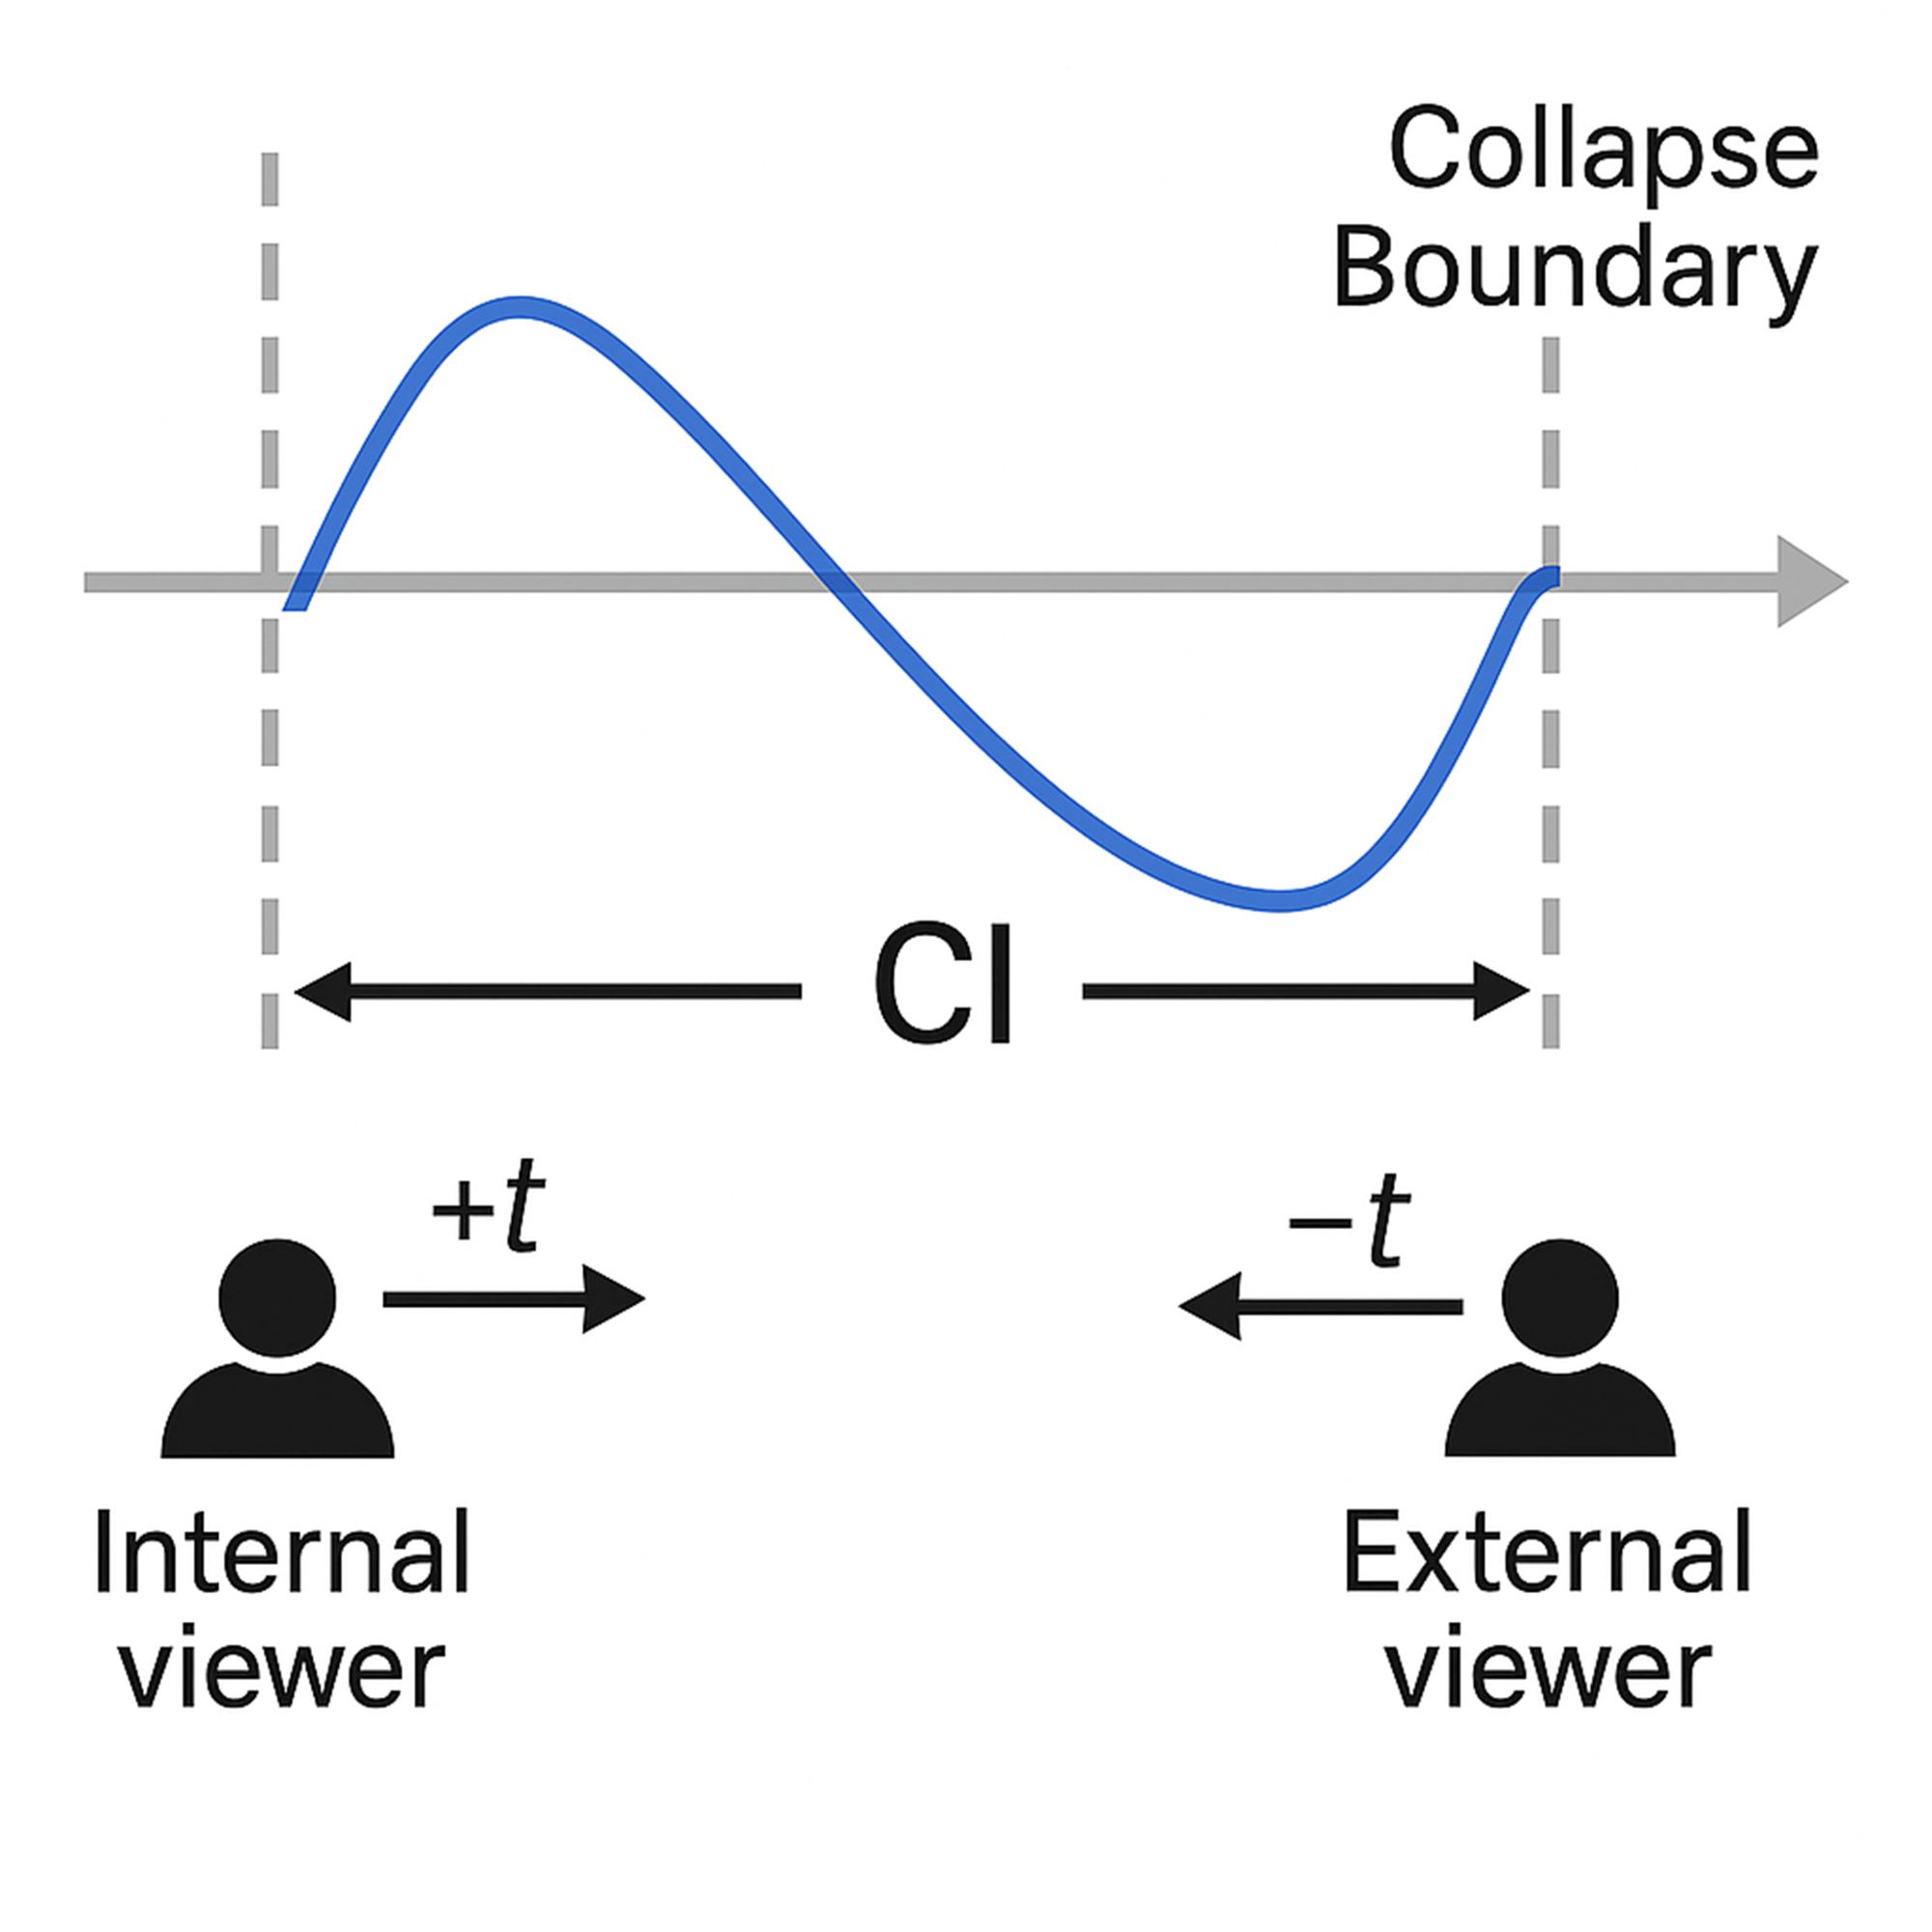
\includegraphics[width=0.50\textwidth]{figures/timing.pdf}
    \caption{Time-relative perspectives in QSD. The internal viewer experiences forward evolution in \( +t \) within the coherence interval (CI), where quantum dynamics unfold causally and reversibly. The external viewer, who only gains access at the Collapse Boundary (CB), must reconstruct prior evolution retrospectively in \( -t \). This dual perspective preserves quantum time symmetry while explaining observational irreversibility as a frame-dependent constraint.}
    \label{fig:timing-perspective}
\end{figure}


In summary, QSD reconciles time symmetry with measurement irreversibility by distinguishing between internal and external perspectives on coherence evolution. The system experiences forward time as it evolves; the observer reconstructs its past only after collapse. There is no contradiction—only a shift in frame. This provides a causal foundation for the quantum arrow of time without requiring thermodynamic assumptions or speculative metaphysics.

%%%%%%%%%%%%%%%%%%%%%%%%%%%%%%%%%%%%%%%%%%
\subsection{Compatibility, Testability, and Limits}
\label{subsec:compatibility}

A central goal of the QSD framework is to preserve the successful predictions of quantum mechanics and quantum field theory while clarifying their domain of applicability and extending their causal structure. The coherence-based model introduced here does not discard the mathematical formalism of quantum theory, but instead embeds it within a structured substrate that defines when and where quantum behavior is permitted. This section outlines how QSD remains compatible with standard theory, identifies points of empirical testability, and defines the limits beyond which quantum formalisms no longer apply without additional substrate structure.

\subsubsection{QM/QFT as a Limiting Case of CI Validity}

Quantum mechanics and QFT are recovered entirely within the Causality Interval \( \mathcal{I}_c \), where the substrate supports phase-coherent structure. Within this domain, unitary evolution, superposition, interference, and entanglement are physically real and mathematically complete. Collapse occurs at the end of \( \mathcal{I}_c \), at the Collapse Boundary \( \mathcal{B}_c \), and measurement becomes meaningful only after this causal resolution.

This places quantum formalism on structurally grounded footing: its validity is exact while the coherence interval remains open, and its termination is not external or observer-driven, but a consequence of causal pacing and envelope constraints. The standard formalism is thus reinterpreted as a limiting case of substrate-supported evolution under coherent conditions.

\subsubsection{Experimental Predictions and Distinctions}

QSD offers several testable predictions that distinguish it from standard quantum theory and interpretations that lack a causal substrate model. These include:

\begin{itemize}
  \item \textbf{Emission asymmetry}: Collapse emissions (QEOs) occurring across substrate gradients may exhibit direction-dependent spectral skew due to anisotropic scalar pacing. This predicts slight asymmetries in photon or particle emission spectra not accounted for by kinematics alone.
  
  \item \textbf{Finite entanglement reach}: Correlation between entangled structures should fail beyond a coherence separation threshold, even in the absence of noise, due to tick desynchronization and phase mismatch across \( L_{\text{coh}} \) boundaries.
  
  \item \textbf{Phase-matched correlation selectivity}: Structures tuned to the same internal geometry may respond collectively to a single QEO if still within the same coherence interval. Multiparty correlation should therefore exhibit a resonance-based response envelope, testable under high timing resolution conditions.
  
  \item \textbf{Null response to antiphase collapse}: If a serialized collapse waveform reaches a partner in geometric antiphase, it may suppress re-lock entirely. This provides a testable prediction in entanglement scenarios involving controlled detuning.
  
  \item \textbf{Collapse-triggered re-lock suppression}: A partner structure receiving a collapse signal may undergo no re-lock event if its own CI has closed or if its phase geometry has been disrupted. This offers a clear falsifiable case for correlated decoherence without classical environmental interaction.
\end{itemize}

These effects can be probed using existing quantum optics and ultrafast detection setups, particularly in time-resolved entanglement studies and phase-controlled interferometry.

\subsubsection{Structural Limits and Future Extensions}

The QSD framework imposes strict structural limits on when quantum formalisms apply. Outside of the coherence interval, wavefunctions no longer represent physically permissible structures. Superposition, interference, and correlation are not destroyed, but become undefined due to lack of substrate support. Similarly, collapse does not terminate the structure, but ends its current configuration. The underlying waveform may persist into future \( \mathcal{I}_c \) intervals, constrained by causal geometry.

Future work may explore the statistical distribution of coherence durations, derive closed-form expressions for tick pacing under substrate tension, and extend this framework to QFT scattering processes, virtual modes, and thermodynamic emergence. These extensions are expected to preserve standard results while anchoring them in a shared physical substrate that restores causal integrity to quantum phenomena.

\smallskip

In summary, QSD is fully compatible with QM and QFT within their domain, and offers clear points of falsifiability based on coherence structure, phase alignment, and causal timing. It does not seek to replace quantum theory, but to supply the structural conditions under which its formalisms arise—and to describe what happens when those conditions break.

%%%%%%%%%%%%%%%%%%%%%%%%%%%%%%%%%%%%%%%%%%


%%%%%%%%%%%%%%%%%%%%%%%%%%%%%%%%%%%%%%%%%%
\section{Conclusion}
%%%%%%%%%%%%%%%%%%%%%%%%%%%%%%%%%%%%%%%%%%

Quantum mechanics and quantum field theory provide some of the most successful predictive tools in the history of science. Yet their interpretive structure remains incomplete: collapse is postulated rather than explained, measurement introduces irreversibility without causal justification, and entanglement correlations challenge both locality and logic. These paradoxes have persisted not because the mathematics is flawed, but because the domain in which it operates has not been clearly defined.

This work presents a resolution: quantum formalism is correct, but applies only within finite causal domains. The framework of General Substrate Theory (QSD) introduces the concept of the \textit{Causality Interval} (CI)—a coherence-permitted span in which quantum evolution proceeds reversibly, consistent with the standard formalism. At the end of each CI lies a \textit{Collapse Boundary} (CB), where coherent evolution terminates and the substrate structurally re-locks the system. If structural offload is required, a \textit{Quantum Emission Opportunity} (QEO) occurs, producing radiation or mass expression through serialized projection of internal geometry.

This minimal causal cycle—CI, CB, QEO—explains quantum behavior without resorting to external triggers or metaphysical postulates. Wavefunctions are real, but temporally bounded. Collapse is not an axiom—it is a consequence of substrate exhaustion. Measurement is not a cause—it is a readout of irreversible commitment. Entanglement is not linkage—it is resonance between phase-compatible structures within shared causal bounds.

Critically, this framework resolves the apparent contradiction between time-symmetric quantum evolution and irreversible measurement. From within the coherence frame, the system evolves forward in time. But from the observer’s point of view—post-collapse—reconstruction of that evolution can only occur retrospectively. Time symmetry is preserved within the CI; causal irreversibility begins at the CB. What appears paradoxical becomes a matter of frame perspective.

The explanatory power of this framework extends beyond collapse. It accounts for emission asymmetry, entanglement decay, multi-structure correlation, and coherence loss under gradient tension—all within a causal architecture grounded in finite structural permission. Quantum behavior emerges not from abstraction, but from constrained evolution within a coherence-governed substrate.

In this view, QM and QFT are not overturned, but anchored. Their equations remain valid—precisely within the limits that the substrate allows. The mysteries of quantum theory are not contradictions; they are the footprints of a deeper causal structure we are only now beginning to see.

\smallskip

QSD does not offer a replacement for quantum theory. It offers an answer to the questions it was never designed to ask:  
\textit{What permits quantum behavior?  
Why does collapse happen?  
And what happens when coherence ends?}

Those answers now begin with structure. And they end—naturally—with causality.


%%%%%%%%%%%%%%%%%%%%%%%%%%%%%%%%%%%%%%%%%%
\vspace{6pt} 

%%%%%%%%%%%%%%%%%%%%%%%%%%%%%%%%%%%%%%%%%%
%% optional
%\supplementary{The following supporting information can be downloaded at:  \linksupplementary{s1}, Figure S1: title; Table S1: title; Video S1: title.}

% Only for journal Methods and Protocols:
% If you wish to submit a video article, please do so with any other supplementary material.
% \supplementary{The following supporting information can be downloaded at: \linksupplementary{s1}, Figure S1: title; Table S1: title; Video S1: title. A supporting video article is available at doi: link.}

% Only used for preprtints:
% \supplementary{The following supporting information can be downloaded at the website of this paper posted on \href{https://www.preprints.org/}{Preprints.org}.}

% Only for journal Hardware:
% If you wish to submit a video article, please do so with any other supplementary material.
% \supplementary{The following supporting information can be downloaded at: \linksupplementary{s1}, Figure S1: title; Table S1: title; Video S1: title.\vspace{6pt}\\
%\begin{tabularx}{\textwidth}{lll}
%\toprule
%\textbf{Name} & \textbf{Type} & \textbf{Description} \\
%\midrule
%S1 & Python script (.py) & Script of python source code used in XX \\
%S2 & Text (.txt) & Script of modelling code used to make Figure X \\
%S3 & Text (.txt) & Raw data from experiment X \\
%S4 & Video (.mp4) & Video demonstrating the hardware in use \\
%... & ... & ... \\
%\bottomrule
%\end{tabularx}
%}

\section*{Statements and Declarations}
\subsection*{Funding}  
The author received no financial support for the research, authorship, or publication of this article.
The author has no relevant financial or non-financial interests to disclose.

\subsection*{Competing Interests}  
The author declares no competing interests.

\subsection*{Author Contributions}  
The author solely conceived, developed, and wrote the manuscript, including all theoretical content, references, and formatting.

\subsection*{Data Availability}  
No datasets were generated or analyzed during the current study. All references are publicly available.

\subsection*{Ethical Approval}  
Not applicable.


%%%%%%%%%%%%%%%%%%%%%%%%%%%%%%%%%%%%%%%%%%
%% Optional

%% Only for journal Encyclopedia
%\entrylink{The Link to this entry published on the encyclopedia platform.}

\abbreviations{Abbreviations}{
The following abbreviations are used in this manuscript:
\\

\noindent
\begin{tabular}{@{}ll}
QSD   & Quantum Substrate Dynamics \\
\( c_s \) & Scalar coherence recovery speed (temporal mode) \\
\( c_t \) & Transverse coherence propagation speed (spatial mode) \\
\( L_0 \) & Baseline coherence length at rest \\
\( L_{\text{coh}}(r) \) & Curvature-stretched coherence support length \\
\( v \) & Apparent velocity relative to substrate \\
\( v_{\text{coh}} \) & Coherence transport velocity \( = \frac{L_{\text{coh}}}{t_{\text{tick}}} \) \\
\( t_{\text{tick}} \) & Local scalar recovery interval (effective time tick) \\
\( t_0 \) & Tick duration at rest (baseline tick) \\
\( \kappa \) & Substrate compliance constant (resistance to boundary deformation) \\
\( \theta(\vec{r}) \) & Local coherence phase at position \( \vec{r} \) \\
\( \rho(\vec{r}) \) & Coherence density distribution \\
\( F_{\text{inertial}} \) & Inertial response force under reconfiguration stress \\
\( P_{\text{offload}}(t) \) & Scalar thermal offload power over time \\
\( \Delta E_{\text{torsion}} \) & Accumulated torsional energy due to rotational strain \\
\( \tau \) & Scalar recovery lag timescale \\
\( \gamma \) & Lorentz factor (compatible structural form) \\
GPS  & Global Positioning System \\
SR   & Special Relativity \\
GR   & General Relativity \\
\end{tabular}

}



%%%%%%%%%%%%%%%%%%%%%%%%%%%%%%%%%%%%%%%%%%
%% Optional
\appendixtitles{no} % Leave argument "no" if all appendix headings stay EMPTY (then no dot is printed after "Appendix A"). If the appendix sections contain a heading then change the argument to "yes".
\appendixstart
\appendix
%%%%%%%%%%%%%%%%%%%%%%%%%%%%%%%%%%%%%%%%%%%%%%%
\section[\appendixname~\thesection]{}
\subsection[\appendixname~\thesubsection]{Substrate Variable Definitions and Tick Pacing}
%%%%%%%%%%%%%%%%%%%%%%%%%%%%%%%%%%%%%%%%%%%%%%
%%%%%%%%%%%%%%%%%%%%%%%%%%%%%%%%%%%%%%%%%%


This appendix provides definitions of key physical quantities used throughout the QSD framework, along with a preliminary expression relating tick pacing to local substrate gradient tension.

\subsubsection{Variable Definitions}

\begin{itemize}
  \item \textbf{\( L_{\text{coh}} \)} — \textit{Coherence Support Length}  
  The maximum spatial extent over which the substrate can support phase-coherent evolution without structural failure. It defines the coherence envelope for a quantum system and governs the size of a valid Causality Interval. \( L_{\text{coh}} \) is not universal; it varies based on local tension, configuration geometry, and substrate saturation.

  \item \textbf{\( c_s \)} — \textit{Scalar Propagation Velocity}  
  The velocity at which scalar reconfiguration (collapse and coherence reset) propagates through the substrate. This value determines how quickly a region of the substrate can recover from offload and support a new coherent structure. It is distinct from the transverse propagation speed \( c \), and is typically much slower, enforcing causal pacing.

  \item \textbf{\( t_{\text{tick}} \)} — \textit{Causality Tick Duration}  
  The duration of one coherence-permitted causal interval for a localized structure. It defines the lifetime of valid quantum evolution prior to collapse:
  \[
  t_{\text{tick}} = \frac{L_{\text{coh}}}{c_s}
  \]
  This duration governs how long a system can maintain coherent evolution before reaching the Collapse Boundary \( \mathcal{B}_c \).

  \item \textbf{\( \mathcal{I}_c \)} — \textit{Causality Interval}  
  The coherence-valid region of spacetime within which unitary evolution and entanglement are physically permitted. Quantum systems evolve freely within \( \mathcal{I}_c \) until coherence becomes unsustainable.

  \item \textbf{\( \mathcal{B}_c \)} — \textit{Collapse Boundary}  
  The boundary condition at the end of \( \mathcal{I}_c \) where the substrate re-locks the system into a committed state, resolving superposition.

  \item \textbf{\( \mathcal{E}_q \)} — \textit{Quantum Emission Opportunity}  
  The optional offload event at the CB where stored tension or waveform structure is serialized into measurable emission (e.g., radiation or particle output). Not all CBs trigger QEOs.

\end{itemize}

\subsubsection{Tick Pacing and Gradient Tension (Preliminary)}

In regions where the substrate experiences a gradient in coherence tension (e.g., due to mass distribution, field distortion, or phase saturation), the effective tick duration may be modulated.

To first approximation, tick duration under a spatially varying coherence tension \( \tau(x) \) may be expressed as:

\[
t_{\text{tick}}(x) = \frac{L_{\text{coh}}(x)}{c_s(x)} \propto \frac{1}{\sqrt{\tau(x)}}
\]

Here, \( \tau(x) \) represents the local substrate tension gradient, which increases with energy density or structural loading. As tension increases, the substrate shortens the allowed coherence interval, forcing earlier collapse.

This relationship may provide a direct mechanism for gravitational redshift, mass variation, or decoherence in strong gradient fields, and is a candidate for further experimental modeling.

\smallskip

Further work will formalize this relationship across curved and layered substrate regions, and relate scalar pacing to effective field curvature without invoking geometric spacetime constructs.

%%%%%%%%%%%%%%%%%%%%%%%%%%%%%%%%%%%%%%%%%%%%%%%
%\section[\appendixname~\thesection]{}
%\subsection[\appendixname~\thesubsection]{APP B}
%%%%%%%%%%%%%%%%%%%%%%%%%%%%%%%%%%%%%%%%%%%%%%%

%\subsubsection{SUB B}

%%%%%%%%%%%%%%%%%%%%%%%%%%%%%%%%%%%%%%%%%%
\isPreprints{}{% This command is only used for ``preprints''.
\begin{adjustwidth}{-\extralength}{0cm}
} % If the paper is ``preprints'', please uncomment this parenthesis.
%\printendnotes[custom] % Un-comment to print a list of endnotes

\reftitle{References}

% Please provide either the correct journal abbreviation (e.g. according to the “List of Title Word Abbreviations” http://www.issn.org/services/online-services/access-to-the-ltwa/) or the full name of the journal.
% Citations and References in Supplementary files are permitted provided that they also appear in the reference list here. 

%=====================================
% References, variant A: external bibliography
%=====================================
% \bibliography{your_external_BibTeX_file}

%=====================================
% References, variant B: internal bibliography
%=====================================

% ACS format
\isAPAandChicago{}{%
\begin{thebibliography}{999}
% Reference 
\bibitem{bush-gst}
Bush, M. (2025). General Substrate Theory: From Substrate Conservation Dynamics to the Emergence of Inertia, Gravity, and Quantization. \textit{Preprints}, 2025070485. \url{https://doi.org/10.20944/preprints202507.0485.v1}
% Reference 
\bibitem{bush2025}
Bush, M. (2025). Quantum Substrate Dynamics (QSD): A Relativistic Field Model of Emergent Mass, Inertia and Gravity. \textit{Preprints}, 2025060988. \url{https://doi.org/10.20944/preprints202506.0988.v1}
% reference
\bibitem{bush-planck-2025}
Bush, M. (2025). Planck’s Constant Physically Derived Through Quantum Substrate Dynamics: A Mode-Ratio and Offload-Based Origin for Quantization and Temporal Structure. \textit{Preprints}, 2024010211. \url{https://doi.org/10.20944/preprints202401.0211.v1}
% Reference 
\bibitem{bush-coherence}
Bush, M. The Coherence Envelope: Defining the Minimum Structural Unit of Action in Quantum Substrate Dynamics. {\em Preprints} {\bf 2025}, \url{https://doi.org/10.20944/preprints202506.2353.v1}.
% Reference 
\bibitem{bush-planck-ep}
Bush, M. Planck Energy as Collapse Limit: A Structural Interpretation of $E_P$ in Quantum Substrate Dynamics. {\em Preprints} {\bf 2025}, \url{https://doi.org/10.20944/preprints202507.0080.v1}.


\end{thebibliography}
}

% Chicago format (Used for journal: arts, genealogy, histories, humanities, jintelligence, laws, literature, religions, risks, socsci)
\isChicagoStyle{%
\begin{thebibliography}{999}
% Reference 1
%\bibitem[Aranceta-Bartrina(1999a)]{ref-journal}
%Aranceta-Bartrina, Javier. 1999a. Title of the cited article. \textit{Journal Title} %6: 100--10.
% Reference 2

\end{thebibliography}
}{}

% APA format (Used for journal: admsci, behavsci, businesses, econometrics, economies, education, ejihpe, games, humans, ijfs, journalmedia, jrfm, languages, psycholint, publications, tourismhosp, youth)
\isAPAStyle{%
\begin{thebibliography}{999}
% Reference 1
%\bibitem[\protect\citeauthoryear{Azikiwe \BBA\ Bello}{{2020a}}]{ref-journal}
%Azikiwe, H., \& Bello, A. (2020a). Title of the cited article. \textit{Journal Title}, \textit{Volume}(Issue), 
%Firstpage--Lastpage/Article Number.

\end{thebibliography}
}{}

% If authors have biography, please use the format below
%\section*{Short Biography of Authors}
%\bio
%{\raisebox{-0.35cm}{\includegraphics[width=3.5cm,height=5.3cm,clip,keepaspectratio]{Definitions/author1.pdf}}}
%{\textbf{Firstname Lastname} Biography of first author}
%
%\bio
%{\raisebox{-0.35cm}{\includegraphics[width=3.5cm,height=5.3cm,clip,keepaspectratio]{Definitions/author2.jpg}}}
%{\textbf{Firstname Lastname} Biography of second author}

% For the MDPI journals use author-date citation, please follow the formatting guidelines on http://www.mdpi.com/authors/references
% To cite two works by the same author: \citeauthor{ref-journal-1a} (\citeyear{ref-journal-1a}, \citeyear{ref-journal-1b}). This produces: Whittaker (1967, 1975)
% To cite two works by the same author with specific pages: \citeauthor{ref-journal-3a} (\citeyear{ref-journal-3a}, p. 328; \citeyear{ref-journal-3b}, p.475). This produces: Wong (1999, p. 328; 2000, p. 475)

%%%%%%%%%%%%%%%%%%%%%%%%%%%%%%%%%%%%%%%%%%
%% for journal Sci
%\reviewreports{\\
%Reviewer 1 comments and authors’ response\\
%Reviewer 2 comments and authors’ response\\
%Reviewer 3 comments and authors’ response
%}
%%%%%%%%%%%%%%%%%%%%%%%%%%%%%%%%%%%%%%%%%%

\isPreprints{}{\PublishersNote{}}

\isPreprints{}{% This command is only used for ``preprints''.
\end{adjustwidth}
} % If the paper is ``preprints'', please uncomment this parenthesis.
\end{document}

